
\chapter{Modelo clásico}

\label{ch:modelo_clasico}

\section{Introducción}
El modelo que planteamos en esta sección pertenece a el modelado considerado clásico realizado en \cite{schaffer}.

Como tenemos gran parte de la dinámica ya planteada, en esta sección, tal y como avanzamos al principio, vamos a presentar la forma en la que se modela la generación de Gli y Ptc (la transcripción génetica) aplicando un enfoque de métodos de termodinámica estadística.

\section{Modelado BEWARE}
 
 
 
 Partimos de dos resultados experimentales que muestran que gli1, gli2 y ptc están regulados transcripcionalmente por la señalización de Shh.
 
  Definimos $K_1$ como la constante de enlace de disociación de equilibrio de Gli y $K_2$ como la constante de enlace de disociación de equilibrio de Gli3 (tanto activador como represor, Gli3R). Los dominios de unión a ADN de todas las formas de Gli están altamente conservados, lo que sugiere que estas las afinidades son similares.
  
  Ante la decisión de que cantidad de enlaces tomar, \cite{schaffer}, para simplificar, suponen que hay el mismo número de posibles enlaces Gli dentro de los
  promotores para Gli y Ptc.
  
  
  El promotor puede existir en numerosos
  estados posibles (promotor vacío, dos Gli  y un Gli3 y el resto de combinaciones de 3 elementos). Ademas la probabilidad de cada estado de unión está determinada por las concentraciones relativas de las tres especies (Gli,Gli3, Gli3R) y sus afinidades de unión al ADN. 
  
  
  Nuestro objetivo es desarrollar el modelo de acuerdo a procedimiento BEWARE, por tanto, para modelar el nivel de activación transcripcional del promotor, calculamos la suma de la probabilidad de cada posible estado del promotor multiplicado por la activación de transcripción de genes que la combinación particular
  induce.
  
  Sin embargo, para ello debemos determinar correctamente  el nivel de activación para un estado dado, con este fin \cite{schaffer,saha} aplican varias reglas:
  En primer lugar la unión del número máximo de activadores transcripcionales (una combinación de Gli y Gli3) produjo un estado con la máxima tasa transcripcional  posible, igual a $(v_{max,G} + r_{bas})$ para el promotor gli.
  
  Aquí donde $v_max$ es la tasa de transcripción inducida máxima y $r_bas$ es igual a la tasa basal de transcripción que se obtendría para un promotor completamente independiente.
  
   Implícita en esta expresión está la suposición de que \cite{schaffer} no tiene en cuenta la dinámica del ARNm, es decir, suponen que cada molécula de ARNm produce un número fijo de proteínas. 
   
   
  A continuación, se permite la posibilidad de unión cooperativa de proteínas al promotor, de forma que el promotor con uno o más factores unidos tuviera una afinidad incrementada por el siguiente factor. A este factor lo denominamos \textit{factor de cooperatividad de unión}$=c$ que habitualmente viene igualado a la unidad ($c=1$).
  
   Además, para cada número de activadores unidos menores que el número máximo de uniones posibles, la velocidad inducida $v_{max, G}$ se multiplica por un factor $e<1$ para poner de manifiesto de una activación transcripcional menor que la máxima. 

Además, para cada represor transcripcional $Gli3R$ unido, la suma $(v_{max, G}+ r_bas)$ se multiplica por el factor de represión $r<1$.
  
Con ambos elementos, multiplicamos la probabilidad de cada estado por la tasa de transcripción de cada estado, sumando los elementos resultantes entre sí y simplificando con ayuda de \cite{sympy}. 
 
 El resultado son dos expresiones relativas al proceso promotor y el proceso de transcripción basal:

 \begin{equation}
  Promoter=\frac{\left(Gli K_{2} + Gli_{3} K_{1}\right) \left(3 K_{1}^{2} K_{2}^{2} e^{2} + 3 K_{1} K_{2} c e \left(Gli K_{2} + Gli_{3} K_{1} + 2 Gli3R K_{1} e r\right) + c^{2} \left(Gli^{2} K_{2}^{2} + 3 Gli Gli3R K_{1} K_{2} e r + Gli_{3}^{2} K_{1}^{2} + Gli_{3} K_{1} \left(2 Gli K_{2} + 3 Gli3R K_{1} e r\right) + 3 Gli3R^{2} K_{1}^{2} e^{2} r^{2}\right)\right)}{K_{1}^{2} K_{2}^{2} \left(3 Gli_{3} K_{1} + 3 Gli3R K_{1} + K_{2} \left(3 Gli + K_{1}\right)\right) + 3 K_{1} K_{2} c \left(Gli K_{2} + Gli_{3} K_{1} + Gli3R K_{1}\right)^{2} + c^{2} \left(Gli K_{2} + Gli_{3} K_{1} + Gli3R K_{1}\right)^{3}}
 \label{promoter_1}
 \end{equation}

 \normalsize
 
 
 \begin{equation}
 Basal=\frac{K_{1}^{2} K_{2}^{2} \left(3 Gli K_{2} + 3 Gli_{3} K_{1} + K_{1} \left(3 Gli3R r + K_{2}\right)\right) + 3 K_{1} K_{2} c \left(Gli K_{2} + Gli_{3} K_{1} + Gli3R K_{1} r\right)^{2} + c^{2} \left(Gli K_{2} + Gli_{3} K_{1} + Gli3R K_{1} r\right)^{3}}{K_{1}^{2} K_{2}^{2} \left(3 Gli_{3} K_{1} + 3 Gli3R K_{1} + K_{2} \left(3 Gli + K_{1}\right)\right) + 3 K_{1} K_{2} c \left(Gli K_{2} + Gli_{3} K_{1} + Gli3R K_{1}\right)^{2} + c^{2} \left(Gli K_{2} + Gli_{3} K_{1} + Gli3R K_{1}\right)^{3}}
 \label{basa_1}
 \end{equation}
 
   
\section{Sistema final}
 Con los operadores BEWARE finalmente calculados podemos ya disponer de el sistema dinámico final que modeliza el sistema de señalización de Shh:
 
 \begin{equation}
 \frac{dGli}{dt} = v_{max,G}Promoter+r_{bas,G}Basal-k_{deg}Gli,
 \label{eq1:1}
 \end{equation}
 
 \begin{equation}
 \frac{dGli_3}{dt} = \frac{r_{g3b}}{Ptc}-Gli_3\left(k_{deg}+\frac{k_{g3rc}}{K_{g3rc}+Signal}\right),
 \label{eq1:2}
 \end{equation}
 
 \begin{equation}
 \frac{dGli3R}{dt}= Gli_3\left(\frac{k_{g3rc}}{K_{g3rc}+Signal}\right)-k_{deg}Gli3R,
 \label{eq1:3}
 \end{equation}
 
 \begin{equation}
 \frac{dPtc}{dt} = v_{max,P}Promoter+r_{bas,P}Basal-k_{degp}Ptc.
 \label{eq1:4}
 \end{equation}
 
\section{Estados estacionarios}
Siguiendo con el estudio estandar que se lleva a cabo en los modelos matemáticos procedemos con un estudio sobre los estados estacionarios que podemos encontrar en nuestro modelo. En primer lugar procedemos afrontando el problema desde una perspectiva analítica. 

Sean las ecuaciones \ref{eq1:1}\ref{eq1:2}\ref{eq1:3}\ref{eq1:4}, si suponemos que éstas se encuentran en un estado estacionario entonces sus cantidades son constantes. Esto implica que su derivada temporal es igual a cero.

Dado que las ecuaciones continen términos complejos, nos interesamos por agruparlas, de manera que los cálculos no sean más sencillo en un primer intento de extraer información:

Por un lado de \ref{eq1:1} y \ref{eq1:4}:

$$\begin{cases} 0 = v_{max,G}Promoter+r_{bas,G}Basal-k_{deg}Gli, \\0= v_{max,P}Promoter+r_{bas,P}Basal-k_{degp}Ptc. \end{cases}$$
Teniendo en cuenta:

$$
r_{bas,G}=\frac{v_{max,G}}{100},r_{bas,P}=\frac{v_{max,P}}{100}
$$

Si igualamos ambas ecuaciones nos queda:
\begin{equation*}
\frac{k_{deg}}{v_{max,G}}Gli=Promoter+\frac{1}{100}Basal=\frac{k_{degp}}{v_{max,P}}Ptc \implies \frac{v_{max,P}k_{deg}}{v_{max,G}k_{degp}}Gli=Ptc
\end{equation*}

 En particular si llamamos $k_{cc}=\frac{v_{max,P}k_{deg}}{v_{max,G}k_{degp}}$:
 \begin{equation}
k_{cc}Gli=Ptc
\label{gli-ptc}
 \end{equation}


Por otra parte, de \ref{eq1:2} y \ref{eq1:3}:



$$\begin{cases} 0 = \frac{r_{g3b}}{Gli}-Gli_3\left(k_{deg}+\frac{k_{g3rc}}{K_{g3rc}+Signal}\right), \\0=Gli_3\left(\frac{k_{g3rc}}{K_{g3rc}+Signal}\right)-k_{deg}Gli3R. \end{cases}$$

Sumando, obtenemos:

\begin{equation}
\begin{split}
0=\frac{r_{g3b}}{Gli}-Gli_3k_{deg}-k_{deg}Gli3R & \implies \frac{r_{g3b}}{Gli}=Gli_3k_{deg}+k_{deg}Gli3R\implies
\\
& \implies \frac{r_{g3b}}{Gli_3k_{deg}+k_{deg}Gli3R}=Gli
\end{split}
\label{gli3gli}
\end{equation}

Con estas cuentas, podemos obtener, en primer lugar, una función de $Signal$\ref{signal} modificada gracias a \ref{gli-ptc}, la llamaremos $Signal_{modificada}$:
\begin{equation}
Signal_{modificada}=\frac{\frac{Shh}{k_{shh}} + 1}{\frac{Shh}{k_{shh}} + 1 + \frac{k_{cc}}{k_{ptc}Gli}}.
\end{equation}

Ahora, sustituimos los valores que tenemos de manera que podamos expresar todas las concentraciones en función de Gli. 

Nuestro obejtivo es intentar hallar los estados estacionarios mediante los puntos fijos entre dos expresiones de Gli. Con ello, usando \ref{gli3gli} nos quedaría:

\begin{equation}
 \frac{r_{g3b}}{Gli}=Gli_3k_{deg}+k_{deg}Gli3R
 \implies Gli_3=\frac{r_{g3b}(K_{g3rc}+Signal_{modificada})}{k_{deg}(K_{g3rc}+Signal_{modificada})Gli}
\label{equgli3}
\end{equation}
 Y de nuevo, por  \ref{gli3gli}:
 
 \begin{equation}
 Gli3R=\frac{r_{g3b}}{k_{deg}Gli}-Gli_3
 \label{equgli3r}
 \end{equation}

Debido a la capacidad de expresar Gli3R y $Gli_3$ con respecto a Gli, podemos obtener la variación de Promoter y Basal directamente con Gli, substituyendo en ellos el valor de Gli3R y $Gli_3$
Con ello, finalmente obtenemos una igualdad cuyos puntos fijos nos darán los posibles estados estacionarios. De \ref{eq1:1} igualado a cero :

 \begin{equation}
 Gli=\frac{v_{max,G}}{k_{deg}}Promoter_{modificado}(Gli)+\frac{1}{100}Basal_{modificado}(Gli)
 \label{final_gli}
 \end{equation}


\section{Simulaciones}

En esta sección vamos a desarrollar todas las simulaciones numéricas llevadas a cabo en el estudio cualitativo del modelo de \cite{schaffer}.
\subsection{Parámetros}
A menos que se especifique lo contrario, para las simulaciones hemos tomado como valores de parametros:
\begin{table}[h]
	\begin{center}
		
		\begin{tabular}{ |p{3cm}||c|p{3cm}|p{3cm}|  }
			\hline
			\multicolumn{4}{|c|}{Tabla de parámetros de \cite{schaffer}  } \\
			\hline
			Parámetro & Valor & Descripción & Fuente\\
			\hline
			$Shh $  & $0-30$    &\tiny{Cantidad de Shh} &   \cite{cambon1}\\
			$k_{Shh}$ &  $ 0.58-2.0nM$  & \tiny{Constante de disociación de los enlaces Ptc-Shh}   & \cite{cambon1}\\
			$k_{Ptc} $ & $8.3\times10^{-11}M$ & \tiny{ Mitad de la máxima concentración de Ptc que inhibe la señal de Smo } &  \cite{cambon1}\\
			$k_{deg}$   &$0.009min^{-1} $ & \tiny{ Constante de degradacion de todas las moleculas Gli } &  \cite{cambon1}\\
			
			$k_{g3rc}$ &  $0.012min^{-1}$  & \tiny{ Constante deconversion de Gli3 en Gli3R} & \cite{schaffer}\\
			$r_{g3b}$ & $1.6\times10^{-19}M^2/min$  & \tiny{ Tasa basal de sintesis de Gli3 }   & \cite{schaffer}\\
			$K_{g3rc}$ & $0.1$ & \tiny{ Constante de sensibilidad de la conversioon a fuerza de la señal }   & \cite{schaffer}\\
			
			$k_{deg_p}$& $0.09min^{-1} $ &  \tiny{constante de degradacion de Ptc} & \cite{cambon1}\\
			
			\hline
		\end{tabular}
		
	\end{center}
	\caption{Tabla de parámetros de \cite{schaffer} }\label{param_2}
\end{table}

\subsection{Variación del operador BEWARE (promoter y basal)}
 \begin{figure}[h]
 	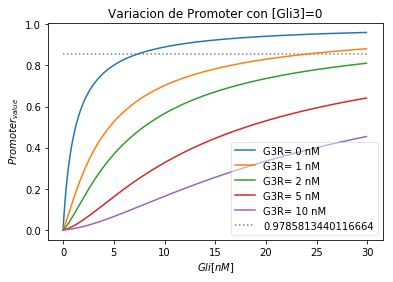
\includegraphics[width=0.8\textwidth]{variacion_promoter}
 	\centering
 	\caption{Variacion del Operador Promoter bajo la variacion de Gli3R }
 	\label{varipro}
 \end{figure}

\begin{figure}[h]
	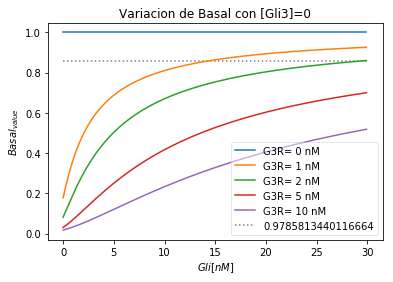
\includegraphics[width=0.8\textwidth]{variacion_basal}
	\centering
	\caption{Variacion del Operador Basal bajo la variación de Gli3R }
	\label{varibas}
\end{figure}

\subsubsection{Reducción de la complejidad del operador}

\begin{figure}[h]
	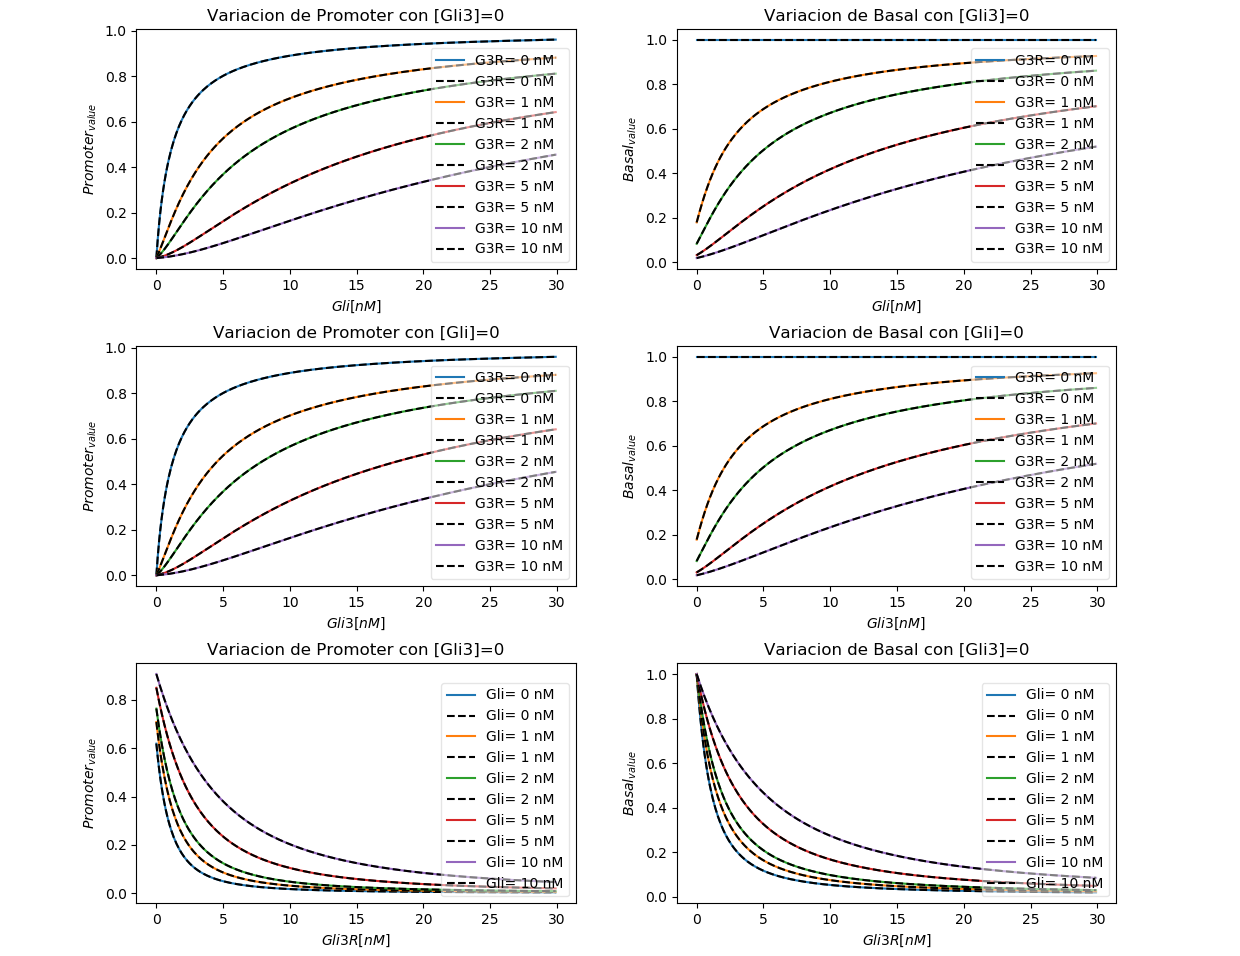
\includegraphics[width=0.8\textwidth]{reduced_form_promoter}
	\centering
	\caption{Comparación numérica de las formas de reducidas de Promoter y Basal (en negro discontinuo) frente a las formas de \cite{schaffer} }
	\label{compara}
\end{figure}

\subsection{Evolución temporal}
Observamos dos interesantes comportamientos según varía la cantidad de $Shh/k_{Shh}=0.1$ en \ref{lai1}, $Shh/k_{Shh}=1.5$ en \ref{lai2}:



 \begin{figure}[h]
 	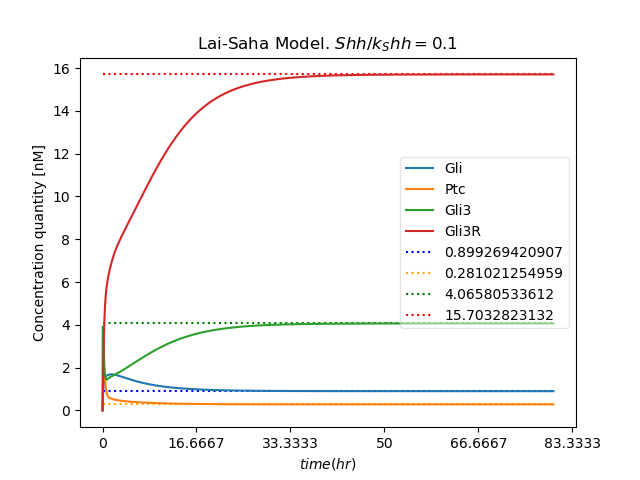
\includegraphics[width=0.8\textwidth]{lai2}
 	\centering
 	\caption{Evolución del modelo \cite{schaffer} con $Shh/k_{Shh}=0.1$ }
 	\label{lai1}
 \end{figure}


\begin{figure}[h]
	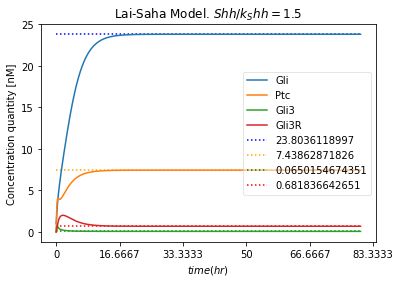
\includegraphics[width=0.8\textwidth]{lai1}
	\centering
	\caption{Evolución del modelo \cite{schaffer} con $Shh/k_{Shh}=1.5$}
	\label{lai2}
\end{figure}

\subsection{Análisis numérico de los estados estacionarios}

\subsection{Diagramas de bifurcación}
\subsubsection{Bifurcación bajo $Shh/K_{Shh}$}
\subsubsection{Bifurcación bajo $r_{g3b}$}
\begin{figure}[h]
	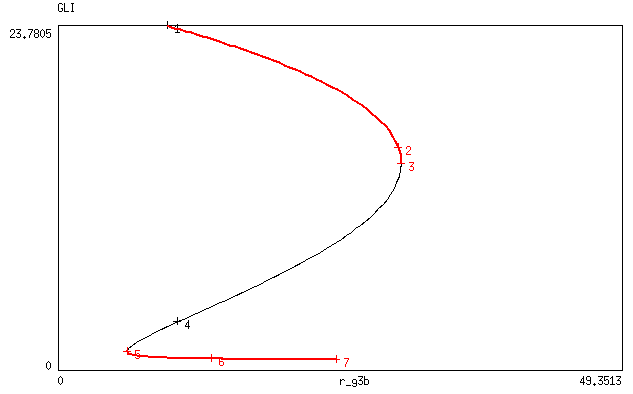
\includegraphics[width=0.8\textwidth]{gliVSr_g3b}
	\centering
	\caption{Diagrama de Bifurcaciónde \cite{schaffer} con $Gli$ frente a $r_{g3b}$}
	\label{lai2}
\end{figure}
\section{Críticas}
Redactando:
\begin{itemize}
	\item erratas en el paper
	\item algunas simplificaciones del modelo
\end{itemize}



